\chapter{Predicting arrival time}
\label{cha:prediction}

\phantom{\gls{gps},\gls{gtfs},\gls{gtfs},\gls{gtfs}}

So far, we have discussed the structure of transit data and its use in constructing a \emph{transit road network} (\cref{cha:data}) through which we model vehicles in real-time using a particle filter to estimate average vehicle speed along roads (\cref{cha:vehicle_model}). These speeds are, in turn, used to update a Kalman filter model of real-time road state (\cref{cha:network_model}). We now have everything needed to begin predicting the arrival time of buses at stops.

In this chapter, we introduce one final state which combines all of the information we have gained thus far. \emph{Trip state} provides a means of combining schedule information with real-time vehicle data to simplify the process of predicting stop arrival times, which also involves the network state and dwell-time information. The first step, therefore, is to estimate trip state (\cref{sec:trip_state}) based on the \gls{gtfs} schedule and estimated vehicle states from \cref{cha:vehicle_model}. Other frameworks have used a similar process, such as \citet{Cathey_2003}, who used a \emph{trip tracker} to prescribe real-time vehicle observations to trip states for use in the \emph{prediction} step.

The remainder of this chapter involves comparing a selection of four models---two using the real-time vehicle and network states, and two others for comparison (including the method currently in use in Auckland). \Cref{sec:prediction_arrival_time} presents the methods before we examine the results of arrival time prediction for a full day of observations for which we know the actual arrival time, allowing us to compare the performance of the methods (\cref{sec:prediction_model_comparison}). Lastly, we discuss the real-time implementation and performance results (\cref{sec:prediction_performance}) and assess the practicality of using a particle filter for arrival time prediction. This chapter focuses on the statistical properties of the prediction methods; practical issues are discussed in \cref{cha:etas}.


\section{Trip state}
\label{sec:trip_state}

At any one time, there are numerous scheduled trips within the transit network we want to obtain the \emph{state} of, which can then be updated with any real-time vehicle or network information, if available. Occasionally there is no vehicle associated with a given trip, so having a trip state makes it possible to combine schedule data with real-time network information to obtain \glspl{eta}. That is, it enables real-time arrival time prediction in the absence of real-time vehicle data.


At any time $t$, we obtain a list of scheduled trips such that the trip's start time $T_\text{start}$ is less than 30~minutes before $t$, and the trip's end time (arrival at last stop) is less than 60~minutes after $t$. The state of each trip within this window is represented by: $\Tript_k$, the time of the previous vehicle observation associated with it (if there is one); $\TripStop_k$, the current stop index; $\TripDep_k$, an indicator of whether the vehicle has departed from that stop; $\TripSeg_k$, the current segment index; and $\SegProg_k$, the progress (as a proportion) along the segment. These are stored in the trip state vector
\begin{equation}
\label{eq:trip_state}
\Tripr_k = \tvec{\Tript_k, \TripStop_k, \TripDep_k, \TripSeg_k, \SegProg_k}.
\end{equation}
The initial state is $\Tripr_0 = \tvec{T_\text{start},0,0,0,0}$. Trips use the same time subscript $k$ as vehicle locations since they are initialised based on the schedule, and then only updated when vehicle data is received.

Estimation of the various state components depends on the type of the most recent observation associated with the trip. The three possible scenarios are:
\begin{enumerate}
\item the last observation was a \emph{trip update} for stop $\TripStop$,
\item the last observation was a \emph{GPS position}, or
\item no data is available for the trip.
\end{enumerate}


\paragraph{Scenario 1:}
On arrival at stop $\TripStop$ at time $\Tript_k$, the trip's state is
\begin{equation}
\label{eq:trip_state_tu}
\Tripr_k =
\begin{cases}
\tvec{\Vtime_k, \TripStop, 0, \TripSeg(s), 0} & \text{if arrival}, \\
\tvec{\Vtime_k, \TripStop, 1, \TripSeg(s), 0} & \text{if departure},
\end{cases}
\end{equation}
where $\TripSeg(s)$ is the segment index of stop $\TripStop$.


\paragraph{Scenario 2:}
Here, the vehicle has completed travel along part of the segment, so the \emph{remaining distance} is needed. From the \pf{} in \cref{cha:vehicle_model}, the segment along which the vehicle is travelling at time $\Tript_k$ is identified as $\TripSeg_k$, and the most recently visited stop is $\TripStop_k$. The proportion of the segment travelled at time $t_k$, $\SegProg_k$, is easily calculated using the vehicle's current distance $\Vdist_k$ and the segment's start distance $\Tsegd_{\TripSeg_k}$ and length $\Tseglen_{\TripSeg_k}$:
\begin{equation}
\label{eq:trip_seg_completed_prop}
\SegProg_k = \frac{\Vdist_k - \Tsegd_{\TripSeg_k}}{\Tseglen_{\TripSeg_k}}.
\end{equation}


\paragraph{Scenario 3:}
There are three main reasons for there being no observations associated with a scheduled trip:
\begin{enumerate}
\item the trip has been cancelled, so no vehicle is servicing the trip, but the cancellation has not been entered into the real-time system;
\item the vehicle is late and has not yet started the trip; or
\item a vehicle is servicing the trip but its \gls{avl} system is either not working or is registered with the wrong trip.\footnote{This happens more often than one might first imagine.}
\end{enumerate}
There is no way to differentiate these three situations without physical investigation, so we always assume there is a bus travelling the route. However, if no bus has been observed, it is desirable to display a warning to passengers so that they are aware and can choose to catch an alternative bus instead.


It is common for passengers waiting at the first stops along a route to have no available \gls{rti} until the bus is a few minutes away. This is because the bus does not register with the server until it has begun the trip. Until this happens, the \gls{dms} displays the default scheduled time, which can be problematic if the bus is late to start the route. In extreme cases, once the scheduled time has passed the service disappears from the \gls{dms}, leaving passengers wondering whether the bus will eventually come, which is why it is necessary to display to commuters if no \gls{rti} is available for a trip.


Additionally, historical data of arrival times can be used in conjunction with the real-time network state to provide a prior estimate of arrival time, which is particularly useful for trips prone to starting late. In these situations, a single prediction is made when first initialising the trip based on historical information. Once the trip is observed (or cancelled) the prediction can be updated. The goal here is not to predict arrival times for unobserved vehicles accurately, but instead to smooth the arrival time estimates at the beginning of a trip's schedule for those situations where the vehicle does finally start its route.

\section{Arrival time prediction methods}
\label{sec:prediction_arrival_time}




\begin{knitrout}\small
\definecolor{shadecolor}{rgb}{0.969, 0.969, 0.969}\color{fgcolor}\begin{figure}

{\centering 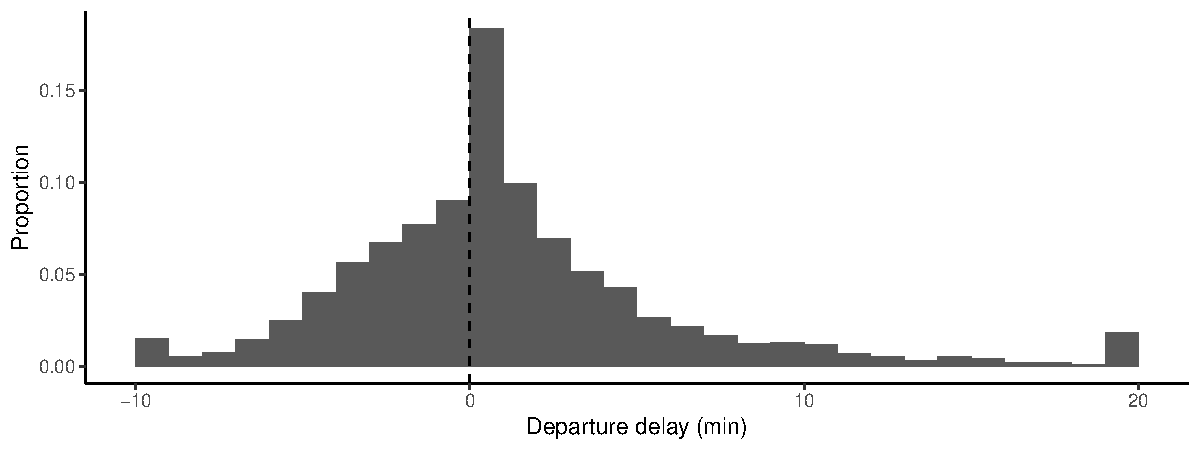
\includegraphics[width=\linewidth]{figure/layover_observance-1} 

}

\caption[Vehicle delays at layover stops truncated to 10~minutes early and 20~minutes late]{Vehicle delays at layover stops truncated to 10~minutes early and 20~minutes late. Negative values indicate non-adherance by drivers, which makes up 40\% of cases.}\label{fig:layover_observance}
\end{figure}


\end{knitrout}

The estimated trip state (and any associated vehicle) and the road network can now be combined to forecast how long it will take for the vehicle to reach all remaining stops along the route. Dwell times can also affect arrival time uncertainty. Some trips have the added complexity of layovers at specific stops---these are common at major points of interest, such as at a mall, or stations where many routes connect so passengers can transfer between services (see \cref{sec:gtfs}). In theory, drivers wait at these stops until the scheduled departure time before continuing the trip; however, in 40\% of cases over two weeks, the driver left before the scheduled departure time, as is demonstrated in \cref{fig:layover_observance}, and 31\% departed more than one minute early.


There are various ways to forecast arrival times, each with associated drawbacks and advantages. This section presents four arrival time prediction methods:
\begin{itemize}
\item \Fpf{} uses the particle filter estimate of vehicle state and the network state to obtain arrival time distributions;
\item \Fnorm{} uses a normal approximation of the vehicle's state, along with the network state and dwell-time distributions;
\item \Fhist{} uses only historical delay data; and
\item \Fsched{} uses the schedule and current real-time delay, as is currently used by \AT{}.
\end{itemize}
The first two use the network state, which is simplified for each route by including only the segments (in order) used by route $r$ with mean and variance
\begin{equation}
\label{eq:route_nw_state}
\RouteNWstate^r =
\begin{bmatrix}
\RouteNWstateseg^r_1 \\
\RouteNWstateseg^r_2 \\
\vdots \\
\RouteNWstateseg^r_L
\end{bmatrix}\quad\text{and}\quad
\RouteNWstatevar^r =
\begin{bmatrix}
\RouteNWstatevarseg^r_{1} & \RouteNWstatecor^r_{1,2} & \cdots &\RouteNWstatecor^r_{1,L} \\
\RouteNWstatecor^r_{2,1} & \RouteNWstatevarseg^r_{2} & \ddots &\RouteNWstatecor^r_{2,L} \\
\vdots & \ddots & \ddots & \vdots \\
\RouteNWstatecor^r_{L,1} & \RouteNWstatecor^r_{L,2} & \cdots & \RouteNWstatevarseg^r_L
\end{bmatrix},
\end{equation}
respectively, where $\RouteNWstateseg^r_{i}$ is the average vehicle speed along the $i$th segment of route $r$, $\RouteNWstatevarseg^r_{i}$ is the variance for the segment, and $\RouteNWstatecor^r_{i,j}$ is the covariance between segments $i$ and $j$. Note that the current implementation does not include segment covariances, but the above setup demonstrates that the model can include them, if available. To simplify notation, I have dropped the $r$ superscript for the remainder of this chapter since only one route is dealt with at any one time.

For bus stop dwell times, we collected two weeks' of data (as was used in \cref{sec:nw_par_est}) and calculated the mean and variance of dwell time for all stops along each trip. It is possible to determine if a bus \emph{did} stop (there is both an arrival and a departure time), but not that a bus \emph{did not} stop. For example, if the bus reports only an arrival time, it is unclear whether this is because the bus truly did not stop, or if it is a deficiency with the data. The bus may not have reported both observations, or, more likely, the polling interval (30 seconds) did not see both of them (Auckland Transport's real-time feed only includes the most recent observation). Therefore, stopping probabilities cannot be estimated from the data, so the same value of $\Prstop_j=0.5$ is used as in \cref{cha:vehicle_model}.


\subsection{Particle filter (\Fpf{})}
\label{sec:prediction_arrival_time_pf}

Each active trip is associated with a single vehicle, itself associated with a set of  $\Np$~particles approximating the vehicle's state. Perhaps the most straightforward method---at least conceptually---of predicting arrival times is to let each particle progress to the end of the route and record its arrival times. Computationally, this is easy to implement but very intensive, significantly increasing iteration time for the application. However, as we no longer need to worry about updating (via importance resampling), we can use a smaller subset of particles, $\Np^\star \leq \Np$, which can be adjusted depending on how many stops there are along the remainder of the route.

\begin{itemize}
\item better argument for using smaller $N$
\item rewrite paragraph below more succinctly (perhaps as a list)
\item for the dwell time stuff, refer back to Ch 3
\end{itemize}


To implement the particle filter forecast method, which we denote \Fpf{}, we take a (weighted) subsample of $\Np^\star$ particles at time $\Vtime_k$, $\tilde\Vstate_k$ (the time of the most recent vehicle observation). For each particle, we calculate the arrival time at each upcoming stop. First, if the particle is at a stop,  the ``remaining travel time'' for the current segment is needed, which we calculate by taking the particle's current speed, adding some noise, and extrapolating to the end of the segment. Having completed the current (partial) segment $j$, the particle's travel time to stop $j$, $\Linkt\vi_j$, is used to estimate the arrival time,
\begin{equation}
\label{eq:particle_arrival_time}
\Tarr\vi_j = \Vtime + \Linkt\vi_j.
\end{equation}
Next, we iteratively add dwell time and travel time for stops and road segments, respectively, until the particle reaches the end of the route; alternatively, we could stop after some number of stops, as we discuss in \cref{sec:prediction_performance}. The dwell time is assumed Gaussian with mean and variance estimated from historical data, $\mu_{\dwell_j}$ and $\sigma_{\dwell_j}$, respectively:
\begin{equation}
\label{eq:prediction_dwell_time}
\begin{split}
\Istop\vi_j &\sim \Bern{\Prstop_j} \\
\pserve\vi_j &\sim \TNormal{\mu_{\dwell_j}}{\sigma_{\dwell_j}}{0}{\infty} \\
\pdwell\vi_j &= \Istop\vi_j \pserve\vi_j
\end{split}
\end{equation}


\begin{itemize}
\item better clarification of terms here
\end{itemize}

When estimating travel time, the particle's speed along each segment is drawn from the network state,
\begin{equation}
\label{sec:particle_travel_time_pred}
\Linkt\vi_j \sim
\Normal{\hat\RouteNWstateseg_j}{
  (P_j + \Delta_j\NWnoise)^2)\wedge\mu_{P_j}
},
\end{equation}
which allows uncertainty to increase for more temporally distant forecasts, with a maximum set by the historical (prior) uncertainty.


Having obtained arrival times for all $\Np^\star$ particles, the predictive distribution for stop $j$---as in \cref{cha:vehicle_model}---is simply
\begin{equation}
\label{eq:particle_predictive_dist}
p(\Tarr_j | \Tripr_k, \RouteNWstate_\Tripr) \approx
\sum_{i=1}^{\Np^\star} \Pwt \dirac_{\Tarr_j\vi}\left(\Tarr_j\right)
= \frac{1}{\Np^\star}\sum_{i=1}^{\Np^\star} \dirac_{\Tarr_j\vi}\left(\Tarr_j\right)
\end{equation}
since all weights are equal. From the particle approximation of the distribution of arrival times we obtain point estimates or quantiles---for example, the mean, median, or a 90\% credible region. As discussed in \cref{app:particle-summaries}, computing quantiles (including the median) is a computationally demanding task for large numbers of particles due to the necessity to sort the particles in order from earliest to latest arrival times---at each stop.

\subsection[Normal approximation]{Normal approximation (\Fnorm{})}
\label{sec:prediction_arrival_time_normal}

Due to the computational demand of the particle filter, significant speed improvements can be obtained by using a normal approximation instead. The network state is a multivariate normal random variable, so the issue lies with stop dwell times having a point mass at zero, resulting in a mixture predictive distribution. For each stop the vehicle passes, there are twice as many components, so after $m$ stops, there are $2^m$ components. However, these regularly converge after a few stops, as shown in \cref{fig:normal_approx}.

\begin{knitrout}\small
\definecolor{shadecolor}{rgb}{0.969, 0.969, 0.969}\color{fgcolor}\begin{figure}

{\centering 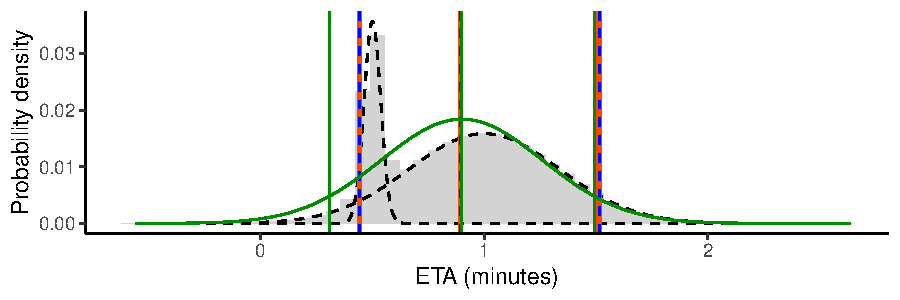
\includegraphics[width=\textwidth]{figure/normal_approx-1} 

}

\caption[Normal approximation for a series of stops ahead]{Normal approximation for a series of stops ahead. The true distribution is shown by the histogram with the underlying components (dashed curves). The vertical lines represent the quantiles computed using the sampled data, the normal mixture (using the optimisation formula), or a single normal approximation.}\label{fig:normal_approx}
\end{figure}


\end{knitrout}

A mixture of normal distributions can approximate the arrival time distribition \citep{Wang_2012} by expressing the mean and uncertainty as vectors $\tilde\mu$ and $\tilde\sigma^2$, respectively, along with a third vector $\tilde\pi$ denoting the $\tilde N$ mixture weights\footnote{We are using the tilde over parameters, e.g., $\tilde x$, to help distinguish them from others used throughout the thesis}, such that
\begin{equation}
\label{eq:ch5:mixture_weight_spec}
\tilde\pi_i > 0, i = 1, \ldots, \tilde N
\text{ and } \sum_{i=1}^{\tilde N} \tilde\pi_i = 1.
\end{equation}
The arrival time at stop $j + n$ is then given by
\begin{equation}
\label{eq:arrival_time_normal_approx}
\Tarr_{j+n} | \tilde\mu, \tilde\sigma^2, \tilde\pi, \RouteNWstate =
\sum_{\ell=j}^{j+n-1} \RouteNWstateseg_\ell +
\sum_{i=1}^{\tilde N} \tilde\pi_i z_i,\quad
z_i \sim \Normal{\tilde\mu_i}{\tilde\sigma^2_i}.
\end{equation}


Each component $i$ has an indicator $I_{im} = \{0,1\}$ of whether or not it stopped at stop $m$, so the total dwell time has mean and variance
\begin{equation}
\label{eq:mixture_dwell_times}
\tilde\mu_i = \sum_{m=j}^{j+n} I_{im} \dwell_m\quad\text{and}\quad
\tilde\sigma_i^2 = \sum_{m=j}^{j+n} I_{im} \dwellvar_m,
\end{equation}
respectively, assuming dwell times at individual stops are independent of each other.

Mixture weights are obtained through the stopping probability at each stop, $\pi_j$:
\begin{equation}
\label{eq:ch5:mixture_weights}
\tilde\pi_i = \prod_{m=j}^{j+n} \tilde p_{im}
\end{equation}
where
\begin{equation}
\label{eq:ch5:mixture_weights2}
\tilde p_{im} =
\begin{cases}
\pi_m & \text{if } I_{im} = 1 \\
1 - \pi_m & \text{otherwise.}
\end{cases}
\end{equation}


The mixture approximation works well for a few stops ahead, but after some time the mixture weights become small and the components combine, as shown in \cref{fig:normal_approx}. To prevent $\tilde N$ from becoming too large, the full distribution is simplified into a single component with mean and variance
\begin{equation}
\label{eq:mixture_mean}
\begin{split}
\E{\Tarr_m | \tilde\pi, \tilde\mu, \tilde\sigma^2, \RouteNWstate} &=
\E{\sum_{\ell=j}^{j+n-1} \RouteNWstateseg_\ell +
  \sum_{i=1}^{\tilde N} \tilde\pi_i z_i} \\
&= \sum_{\ell=j}^{j+n-1} \E{\RouteNWstateseg_\ell} +
  \sum_{i=1}^{\tilde N} \tilde\pi_i \E{z_i} \\
&= \sum_{\ell=j}^{j+n-1} \hat\RouteNWstateseg_\ell +
  \sum_{i=1}^{\tilde N} \tilde\pi_i \tilde\mu_i
\end{split}
\end{equation}
and
\begin{equation}
\label{eq:mixture_variance}
\begin{split}
\Var{\Tarr_m | \tilde\pi, \tilde\mu, \tilde\sigma^2, \RouteNWstate} &=
\Var{\sum_{\ell=j}^{j+n-1} \RouteNWstateseg_\ell +
  \sum_{i=1}^{\tilde N} \tilde\pi_i z_i} \\
&= \sum_{\ell=j}^{j+n-1} \Var{\RouteNWstateseg_\ell} +
  \sum_{i=1}^{\tilde N} \tilde\pi_i^2 \Var{z_i} \\
&= \sum_{\ell=j}^{j+n-1} \hat\RouteNWstatevarseg_\ell +
  \sum_{i=1}^{\tilde N} \tilde\pi_i \tilde\sigma_i^2
\end{split}
\end{equation}
respectively, assuming segment travel time and dwell time are independent---assuming otherwise makes this model impossible to work with; indeed, this model versus the particle filter (which makes no such assumption) is effectively testing the viability of this assumption.


An optimisation is used to obtain quantiles $q_\alpha$ such that
\begin{equation}
\label{eq:mixture_quadratic}
\left[
  p\left(\alpha \leq \Tarr_m | \tilde\pi, \tilde\mu, \tilde\sigma^2, \RouteNWstate\right) - q_\alpha
\right]^2 = 0.
\end{equation}
This is straightforward using Brent's Algorithm \citep{Brent_1971}, implemented in the Boost \textsf{C++} library.

When the 2.5\%, 50\%, and 97.5\% quantiles for the single approximation are within 30~seconds of the same quantiles computed for the mixture distribution, the mixture is replaced with one single component with mean and variance defined in \cref{eq:mixture_mean,eq:mixture_variance}. In some situations, the mixture may not converge into a single distribution quick enough, so to prevent the number of components $\tilde N$ from exceeding $2^8=256$, all components with weights less than a predefined threshold (we used $\frac{1}{2}\max_i(\pi_i)$) are combined into a single component.


%%%%%%%%%%%%%%%%%%%%%%%%%%%%%%%%%%%%%%%%%%%%%%%%%%%%%%%%% Historical data
\subsection{Historical arrival delays (\Fhist{})}
\label{eq:prediction_arrival_historical}

Another way to make predictions is to use historical data instead of real-time. We collected two weeks of data and recorded arrival time delays by stop and route to obtain a distribution which can then be used to make predictions. The arrival time at stop $j$ along route $r$ has an average delay of $\bar d_{rj}$ seconds with variance $D_{rj}^2$, so the predicted arrival time at stop $j$ on route $r$ with scheduled arrival time $S_{rj}$ is
\begin{equation}
\label{eq:arrival_pred_historical}
\hat\Tarr_{j} \sim \Normal{S_{rj} + \bar d_{rj}}{D_{rj}^2}.
\end{equation}


%%%%%%%%%%%%%%%%%%%%%%%%%%%%%%%%%%%%%%%%%%%%%%%%%%%%%%%%% Schedule + delay
\subsection{Schedule delays (\Fsched{})}
\label{eq:prediction_arrival_sched_delay}

The currently deployed prediction method uses the scheduled arrival time at stop $j$ along route $r$, $S_{rj}$, along with the arrival or departure time at the most recently visited stop, $T_{rm}$, giving a current delay, in seconds, of
\begin{equation}
\label{eq:sched_cur_delay}
d_{r} = T_{rm} - S_{rm}.
\end{equation}
The arrival time is then predicted as
\begin{equation}
\label{eq:sched_pred_arr}
\hat\Tarr_{rj} = S_{rj} + d_r.
\end{equation}
Note, however, that if a trip has not yet been observed, the default delay is $d_r = 0$, regardless of whether or not there is a vehicle servicing it, the vehicle is running late, or the trip has been cancelled altogether.

\section{Assessing predictive performance}
\label{sec:prediction_model_comparison}


To compare the four prediction methods, we implemented the first two in the \textsf{transitr} application and, using a single day of data, run the program, storing all arrival time estimates, the uncertainty, as well as the 5\% and 90\% quantiles\footnote{Initially we used a symmetric 95\% prediction interval, but this was often highly skewed by a few very late particles.}. The actual (reported) arrival times are then used to compare the accuracy of each method. For the historical data, we compare the mean with the actual arrival time. For the schedule-delay method, the arrival time for all upcoming stops was predicted after each new observation, and the prediction error computed.

\begin{itemize}
\item yes, rewrite the above para to make more sense please.
\item and, the below might need some more words about MAE/MAPE \ldots
\end{itemize}

We used \gls{rmse}, \gls{mae}, and \gls{mape} as comparison criteria (see \cref{app:error-functions}).
\Gls{rmse} is the mean squared difference (in seconds) between the predicted and actual arrival times. Of course, since predictions change over time, we also compute \gls{rmse} by \emph{time until (actual) arrival}, allowing us to compare the models at different time points, as well as by stop sequence and time of day.


Another criteria we are interested in is the \gls{picp}, which is only available for the three methods for which we can construct an 85\% \gls{ppi}: for the particle filter, this is achieved by sorting the particles in order of arrival time, and then taking the $\lfloor q_\text{lower} N^\star\rfloor^{\text{th}}$ particle as the lower bound, and the $\lceil q_{\text{upper}} N^\star\rceil^{\text{th}}$ particle as the upper bound (more details in \cref{app:particle_summaries}). For the 85\% interval, we used $q_\text{lower} = 0.05$ and $q_\text{upper} = 0.9$. For the normal approximation and historical arrival methods, the inverse \gls{cdf} provides the required quantiles. The results are displayed in \cref{tab:model_results_rmse} and \cref{fig:model_results_rmse_time,fig:model_results_rmse_stopn,fig:model_results_rmse_timeofday} (described in \cref{sec:prediction_model_comp_stats}).


\begin{itemize}
\item predictive power, or `reliability'?
\end{itemize}

Additionally, we also want to compare the predictive power of the various forecast methods, namely \emph{the probability of arriving before the bus}, and hence not missing it, as well as the expected waiting time given a passenger arrives at the stop by a certain time. In table \cref{tab:model_results_pr_miss} and \cref{fig:model_results_pr_gtfs,fig:model_results_pr_time,fig:model_results_pr_stop,fig:model_results_pr_timeofday}, we use the point estimate (mean or median, depending on the forecast method), as well as the 5\% quantile, and for each calculate the probability that the bus arrives after the specified time. We also calculate the expected waiting time for a passenger arriving at a certain time \emph{and the bus arrives after the specified time} (i.e., the passenger catches the bus). \Cref{sec:prediction_model_comp_probs} discusses these results.






\begin{knitrout}\small
\definecolor{shadecolor}{rgb}{0.969, 0.969, 0.969}\color{fgcolor}\begin{table}

\caption{\label{tab:model_results_rmse}Predictive model comparison of RMSE and MAE, in seconds, MAPE (\%), and PICP (\%).}
\centering
\fontsize{8}{10}\selectfont
\begin{tabular}[t]{lrrrr}
\toprule
  & RMSE (s) & MAE (s) & MAPE (\%) & PICP (\%)\\
\midrule
\Fpf{}: Particle filter & 232 & 146 & 19 & 77\\
\Fnorm{}: Normal approximation & 489 & 349 & 38 & 91\\
\Fhist{}: Historical delays & 244 & 166 & 47 & 84\\
\Fsched{}: Schedule-delay & 238 & 164 & 27 & \\
\bottomrule
\end{tabular}
\end{table}


\end{knitrout}




\subsection{Comparing the accuracy of arrival time prediction}
\label{sec:prediction_model_comp_stats}

The accuracy measurements (\gls{rmse}, \gls{mae}, and \gls{mape}) shown in \cref{tab:model_results_rmse} immediately show that the normal approximation (\Fnorm{}) estimates are, on average, about half as accurate as the other methods. Overall, the \pf{} (\Fpf{}) demonstrates the greatest accuracy by all criteria, indicating that its estimates are (on average) closer to the true value in both absolute and relative terms. The historical delays approach (\Fhist{}) has similar accuracy to the schedule-delay approach (\Fsched{}) in absolute terms (\gls{rmse} and \gls{mae}), but the least accurate over all in realtive terms (\gls{mape}), indicating that it has poorer accuracy for short-term forecasts; this is not surprising as it uses purely historical data, so \rt{} information about vehicle location and network state are ignored.


As for the \gls{picp}, the theoretical coverage is 85\%. \Fpf{} seems to underestimate arrival time uncertainty, which indicates that not enough uncertainty is being captured by the model: this could be any combination of dwell time, travel time, or the unknown. Conversely, \Fnorm{} overestimates uncertainty by about 5\%. \Fhist{} has close to the desired \gls{picp}, which demonstrates that arrival time delays at each stop show a certain level of consistency.



From the simple, overall summary in \cref{tab:model_results_rmse}, it is difficult to comment on the relative performance of the methods, except that the normal approximation seems to be ill-suited to the task. However, this was not unexpected: throughout the previous chapters, we have commented on the non-Gaussian nature of transit vehicle state. We now explore the effects of time until arrival, stop sequence, and time of day on prediction accuracy.


\subsubsection{Time until actual arrival}

We would expect arrival time predictions for a given stop to become more accurate as the bus approaches it. To assess this, arrival time estimates for binned into one-minute intervals, and for each interval the same summary statistics were estimated and displayed in \cref{fig:model_results_rmse_time}. Note the use of log scales for \gls{rmse}, \gls{mae}, and \gls{mape}.



\begin{knitrout}\small
\definecolor{shadecolor}{rgb}{0.969, 0.969, 0.969}\color{fgcolor}\begin{figure}
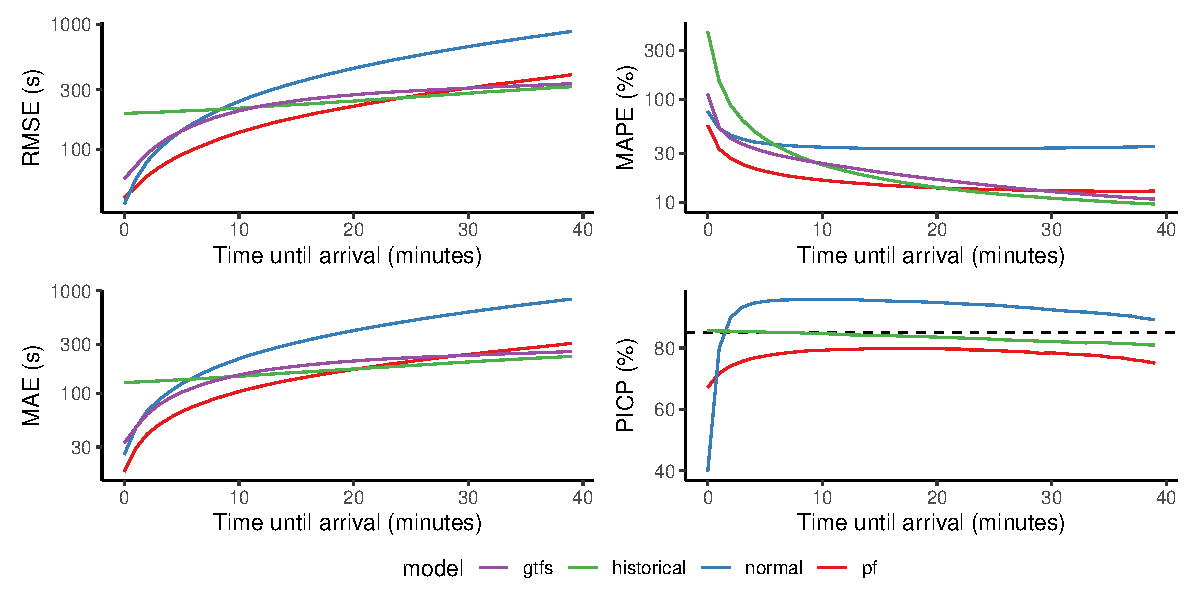
\includegraphics[width=\textwidth]{figure/model_results_rmse_time-1} \caption[Model comparative statistics as a function of time until arrival]{Model comparative statistics as a function of time until arrival. Note the log-scale for RMSE, MAE, and MAPE.}\label{fig:model_results_rmse_time}
\end{figure}


\end{knitrout}


The \gls{rmse} and \gls{mae} for all methods increase with time until arrival as expected, but the rate at which this occurs varies. The three methods that use \rt{} information (\Fpf{}, \Fnorm{}, and \Fsched{}) demonstrate small absolute error when the bus is near, which increases the farther out the bus gets, while \Fhist{} shows a more constant error and far poorer accuracy when the bus is less than 50--10~minutes away. \Fpf{} has the lowest error up until 20~minutes before arrival, and has greater accuracy than \Fsched{} up until 25--30~minutes. This indicates that the current delay is only a useful predictor when the bus has almost arrived, and that accounting for \rt{} traffic conditions \emph{does} improve the accuracy of arrival time prediction. \Fnorm{} quickly shows large prediction errors for all but the nearest buses.




The \gls{mape} for all methods decreases with time until arrival, with \Fhist{} showing the highest relative error when the bus is less than about 5~minutes away. \Fnorm{} remains fairly constant with a large relative error (about 50\%).Again for the first 20~minutes, \Fpf{} has the smallest relative error, and is better than \Fsched{} up until the bus is 25--30~minutes away. After 30~minutes, \Fpf{} seems to converge with slightly lower accuracy than \Fhist{} and \Fsched{}, which appear to be continue improving accuracy after the 40~minute cut-off; however, 89\% of routes in Auckland are less than one hour, so the number of arrival time predictions being made that are greater than 40~minutes becomes small (predictions are only made once the trip starts).


The \gls{picp} is not available for \Fsched{} since that method only provides point estimates. The coverage for the three remaining methods is reasonably constant across time until arrival \cref{fig:model_results_rmse_time}. As we saw earlier, \Fpf{} underestimates uncertainty, resuling in lower than expected coverage, and \Fnorm{} overestimates uncertainty for all times greater than a few minutes. \Fhist{} shows good coverage, although this drops off slightly as time until arrival increases, which could indicate that arrival times for later stops along long routes (since these are the only ones with times until arrival this large) are prone to more variability.




\subsubsection{Stop sequence}

Similarly to time until arrival, we grouped results by stop sequence---skipping the first stop since arrival times are only predicted once the bus begins the trip---and computed the familiar summary statistics, which are displayed in \cref{fig:model_results_rmse_stopn}. Note that stop sequence and time until arrival are correlated, since early stops along a route seldom have long until the bus arrives (once it has begun), and that only 8\% of ~trips have more than 50~stops.


\begin{knitrout}\small
\definecolor{shadecolor}{rgb}{0.969, 0.969, 0.969}\color{fgcolor}\begin{figure}
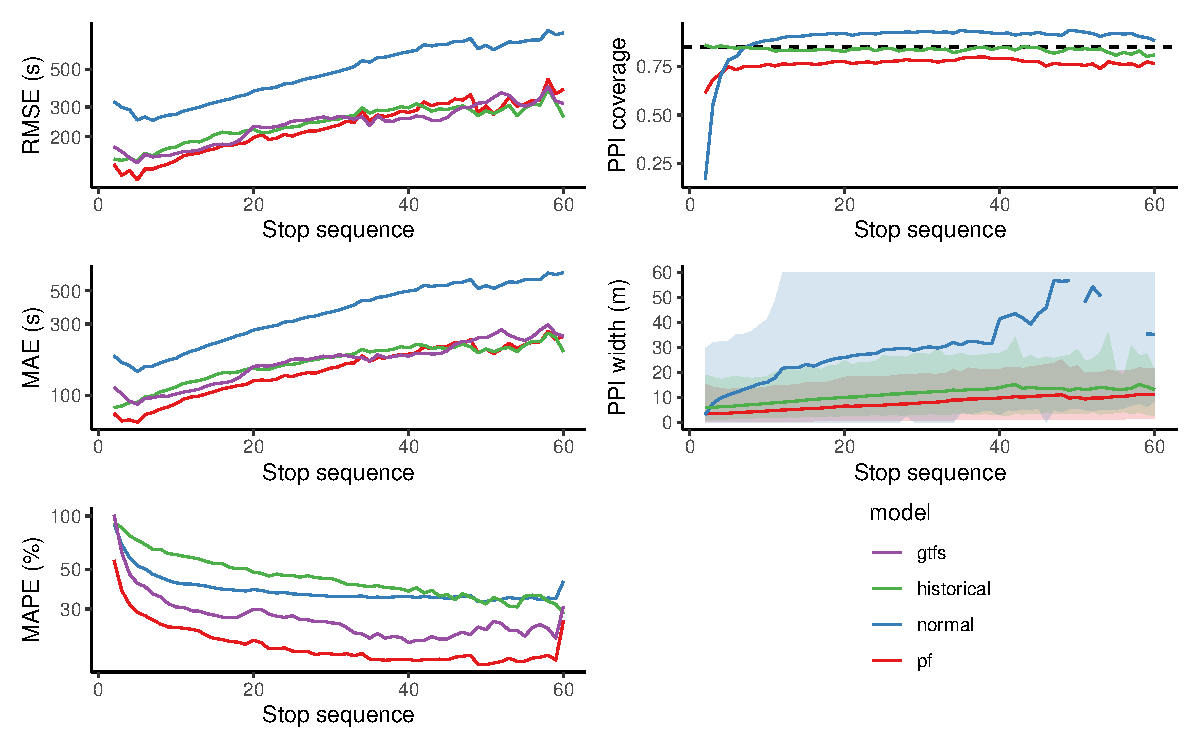
\includegraphics[width=\textwidth]{figure/model_results_rmse_stopn-1} \caption[Model comparative statistics as a function of stop sequence]{Model comparative statistics as a function of stop sequence.}\label{fig:model_results_rmse_stopn}
\end{figure}


\end{knitrout}

The \gls{rmse} and \gls{mae} increase for all models up until stop 50, after which point only few routes have that many stops, so there is increased variability between consecutive stops. As before, \Fnorm{} shows much higher errors than the other three methods, and \Fpf{} shows slightly better prediction accuracy than \Fhist{} and \Fsched{} up until about stop 30, at which point there is no clear difference between these three methods. However, in terms of relative error (\gls{mape}), \Fpf{} outperforms all the others over all stops, while \Fhist{} shows the poorest accuracy particularly for early stops.


The \gls{picp} show much the same trend as before, again not unexpected due to the relationship between stop sequence and time until arrival. \Fpf{} underestimates uncertainty at all stops, while \Fnorm{} overestimates for all but the first few stops---it performs quite poorly for those. \Fhist{} has the desired coverage for all stops.



\subsubsection{Time of day}

We grouped observations into 15~minute intervals over the day and calculated the summary statistics for each prediction method. The results, displayed in \cref{fig:model_results_rmse_timeofday}, differ quite significantly from those seen previously, as we now see a strong peak-hour effect: in the morning there is a single peak (school and work begin at about the same time) at around 8~am, whereas in the evening there are two smaller peaks: one for schools at about 3~pm, and another for workers at around 5~pm.


\begin{knitrout}\small
\definecolor{shadecolor}{rgb}{0.969, 0.969, 0.969}\color{fgcolor}\begin{figure}
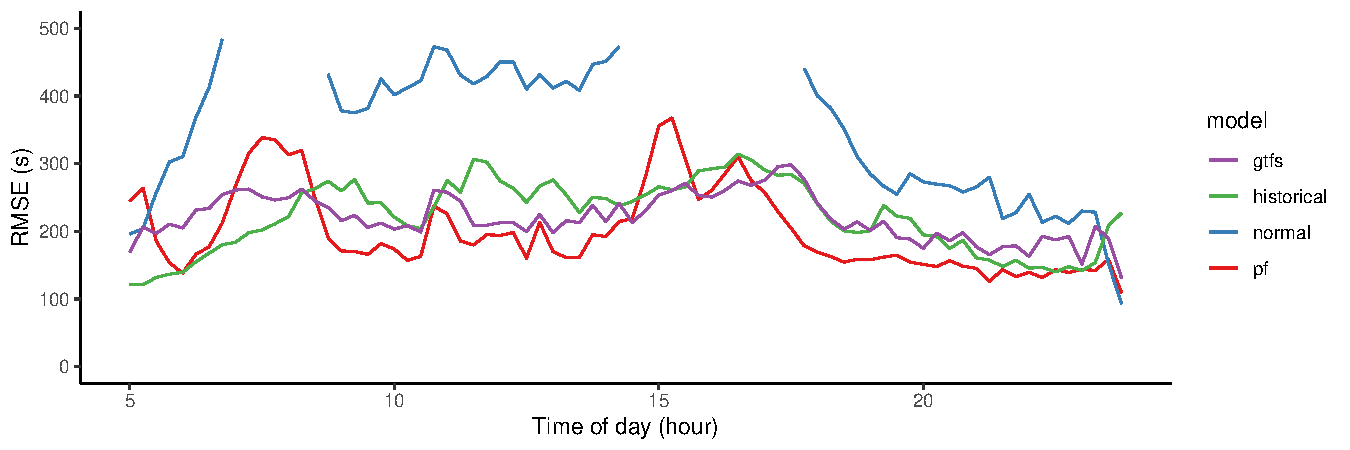
\includegraphics[width=\textwidth]{figure/model_results_rmse_timeofday-1} \caption[Model comparative statistics as a function of time of day]{Model comparative statistics as a function of time of day.}\label{fig:model_results_rmse_timeofday}
\end{figure}


\end{knitrout}

During off-peak (that is, between about 9:30~am and 2:30~pm) \Fpf{} shows the smallest absolute error (\gls{rmse} and \gls{mae}), with \Fhist{} and \Fsched{} showing slightly larger errors. Again, \Fnorm{} shows much poorer accuracy (again, note the log scale). During peak times, all methods show an increase in prediction error as traffic conditions worsen and become more unreliable. \Fsched{} is least affected by this effect since the schedules take, to some extent, peak congestion into account, while the current implementation of our method only uses the \emph{current} traffic state; however, as discussed in \cref{sec:nw_hist_model}, improvements should be possible once a better forecasting method has been implemented.

In terms of relative error (\gls{mape}), we still see the peak effect, but it is much less accentuated, and now \Fpf{} demonstrates the best accuracy throughout the day. This would indicate that much of the absolute error comes from longer-term predictions (when the bus is far away), when traffic has more opportunity to get better or worse: all commuters will be all too familar with how quickly congestion can build. \gls{mape} for \Fsced{} and \Fhist{} show little effect at all of peak hour.


Finally, we look to \gls{picp}, where we can truly see the effect of peak traffic on arrival time predictions, particularly those made using our particle filter. During off-peak, \Fpf{} has very close to the desired coverage of 85\%; during peak time, however, coverage drops quite significantly. This will be due to travel times increasing quickly as congestion builds, meaning initial predictions are too early, and then travel times decreasing again once peak time has passed, and predictions made will be too late. This indicates that, while our \pf{} seems to be able to accurately estimate travel times, it would benefit from the forecasting improvement\footnote{Which we were, unfortunately, unable to complete at this time.}.




\subsection{Assessing the reliability of arrival time prediction}
\label{sec:prediction_model_comp_probs}

\Gls{rmse}, \gls{mae}, and \gls{mape} measure the predictive accuracy of the methods, but do not account for the costs associated with inaccurate predictions. In this section, we evaluate the \emph{reliability} of arrival time distributions by examining
\begin{enumerate}
\item the wait time at the bus stop, and
\item the probability of missing the target bus.
\end{enumerate}
In most cases, the latter incurs a much greater cost, but depends entirely on time until the \emph{next} bus arrival: for high-frequency routes, this will be small; for low-frequency ones, however, it can become quite high\footnote{Some routes only run hourly!}. In this section, we do not differentiate between high and low-frequency routes (we do in \cref{sec:eta_estimates}, however).


The three statistics we compare across the methods are:
\begin{itemize}
\item $\mathbb{P}_m = \Pr{\Varr_m \geq \hat\Tarr_m}$, the probability that the vehicle arrives after the point estimate, $\hat\Tarr_m$, indicating that were a passenger to arrive at the stop by $\hat\Tarr_m$, they would catch the bus with probability $\mathbb{P}_m$;
\item $\mathbb{P}_\ell = \Pr{\Varr_m \geq \hat\alpha_{m,\text{lower}}}$, the probability that the vehicles arrives after the lower bound of the \gls{ppi}; and
\item $\mathbb{E}_\ell = \E{\Varr_m - \hat\alpha_{m,\text{lower}} | \Varr_m \geq \hat\alpha_{m,\text{lower}}}$, the expected waiting time for a passenger arriving at the lower predictive bound, given that the bus arrives after it (that is, conditional on catching the bus).
\end{itemize}


\begin{knitrout}\small
\definecolor{shadecolor}{rgb}{0.969, 0.969, 0.969}\color{fgcolor}\begin{table}

\caption{\label{tab:model_results_pr_miss}The probability of catching a bus given a passenger arrives by the mean/median ($\mathbb{P}_m$) and lower quantile ($\mathbb{P}_\ell$), along with the expected waiting time, in minutes, given arrival by the lower quantile, for each of the for forecast methods.}
\centering
\fontsize{8}{10}\selectfont
\begin{tabular}[t]{lrrrl}
\toprule
  & $\mathbb{P}_m$ (\%) & $\mathbb{P}_\ell$ (\%) & $\mathbb{E}_\ell$ (m) & 95\% CI\\
\midrule
\Fpf{}: Particle filter & 64 & 93 & 4.4 & 0.2--16.6\\
\Fnorm{}: Normal approximation & 96 & 98 & 20.9 & 1.2--63.7\\
\Fhist{}: Historical delays & 54 & 98 & 7.1 & 0.7--20.8\\
\Fsched{}: Schedule-delay & 38 &  &  & \\
\bottomrule
\end{tabular}
\end{table}


\end{knitrout}



The overall results are displayed in \cref{tab:model_results_pr_miss}. If a passenger, at any time, looks at the \gls{eta} of their bus \emph{once} and arrives at the stop by the indicated time, then using \Fpf{} their probability of catching the bus is almost double that of using \Fsched{}. Using \Fhist{}, then (not surprisingly) $\mathbb{P}_m$ is about 50\%; \Fnorm{} is over 95\% which indicates that it is underestimating arrival times.



The concept behind examining the accuracy of the lower quantile, $\mathbb{P}_\ell$, is that this value should give passengers the best chance of catching the bus. We used the 2.5\% quantile for the lower estimate, so we would expect the bus to arrive after the predicted time 97.5\% of the time. This is the case for \Fnorm{} and \Fhist{}, but \Fpf{} has a slightly lower probability that expected. Associated with the lower bound is the expected wait time until the bus actually arrives, conditional on not having missed it ($\mathbb{E}_\ell$). \Fpf{} has the shortest expected wait followed closly by \Fhist{}, while the wait time using \Fnorm{} is about four times as long as with \Fpf{}.



Since \Fsched{} provides only a point estimate, we cannot compare it directly to the other methods, in particular \Fpf{}. To do so, we can \emph{indirectly} compare these methods by proposing a passenger arrives $x$~minutes before the stated arrival time (by \Fsched{}) and calculating the probability of capture and expected wait time. The resulting curves are shown for a range of times (arriving 4--12~minutes before the stated arrival) in \cref{fig:model_results_pr_gtfs}, with the values for the other three methods overlaid with dashed lines.



\begin{knitrout}\small
\definecolor{shadecolor}{rgb}{0.969, 0.969, 0.969}\color{fgcolor}\begin{figure}

{\centering 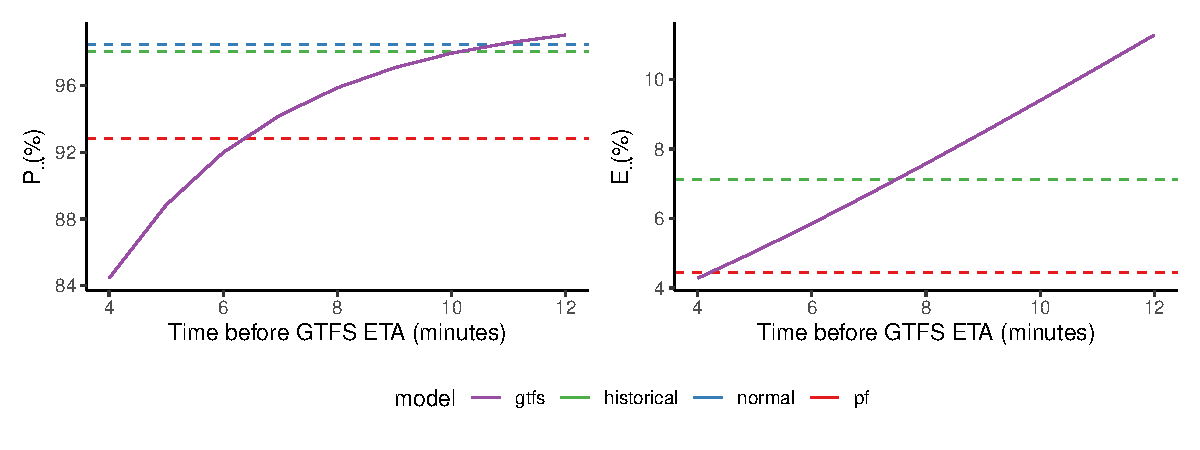
\includegraphics[width=\textwidth]{figure/model_results_pr_gtfs-1} 

}

\caption[GTFS equivalent]{GTFS equivalent}\label{fig:model_results_pr_gtfs}
\end{figure}


\end{knitrout}



First let us consider the probability of the bus arriving after the estimated arrival time, $\mathbb{P}_\ell$. Based on the data collected, a passenger would need to arrive at least 10~minutes before the stated \gls{eta} (by \Fsched{}) to have a 97.5\% probability of catching the bus. To obtain the same probability as \Fpf{}, this would be 6~minutes before arrival. Now we can compare the expected waiting time: to achieve the targetted 97.5\% chance of catching the bus, the passenger would arrive 10 minutes before the stated \gls{eta}, which has an expected waiting time of about 9~minutes. Or, arriving 6~minutes before, the expected wait time drops to almost 6~minutes, which is greater than the expected wait time under \Fpf{} of just over 4~minutes.


We could also examine this the opposite way, and match the expected waiting time with that of \Fpf{}. In this case, a passenger would need to arrive no more than 4~minutes before the stated arrival time, which would give them an 85\% chance of catching the bus. For the remainder of this section, we use 6~minutes before the specified \gls{eta} to obtain a lower bound for \Fsched{}, and compare the probabilities as a function of time until arrival, stop sequence, and time of day.



\subsubsection{Time until arrival}

\Cref{fig:model_results_pr_time} shows $\mathbb{P}_m$, $\mathbb{P}_\ell$, and $\mathbb{E}_\ell$ computed in one-minute intervals for each of the four models. We see that the probability that the vehicle arrives after the estimate is reasonably constant, with a slight decrease as the bus nears the stop; however, the four methods are distinct from each other, yielding the same conclusion as before \textcolor{red}{(be more specific)}.

As for $\mathbb{P}_\ell$, displayed in \cref{fig:model_results_pr_time2}, we see a different trend: $\FM_1$ and $\FM_3$ increase the further out the vehicle is, while in $\FM_4$ the probability decreases. Clearly, this is because we have chosen a fixed lower bound. When the vehicle is less than 15 minutes out, arriving 6~minute before the schedule-delay estimate results in a higher probability of catching the bus than the particle filter because the width is greater.


Finally, we look at the expected waiting time, given a passenger arrives at the lower bound \emph{and} the bus arrives sometime after, which is displayed in \cref{fig:model_results_pr_time}. The particle filter has a consistently shorter waiting time, though by about 30~minutes out the three methods excluding the normal approximation are approximately the same. We can see that the expected waiting time for $\FM_4$ is more or less independent of time until arrival.



\begin{knitrout}\small
\definecolor{shadecolor}{rgb}{0.969, 0.969, 0.969}\color{fgcolor}\begin{figure}
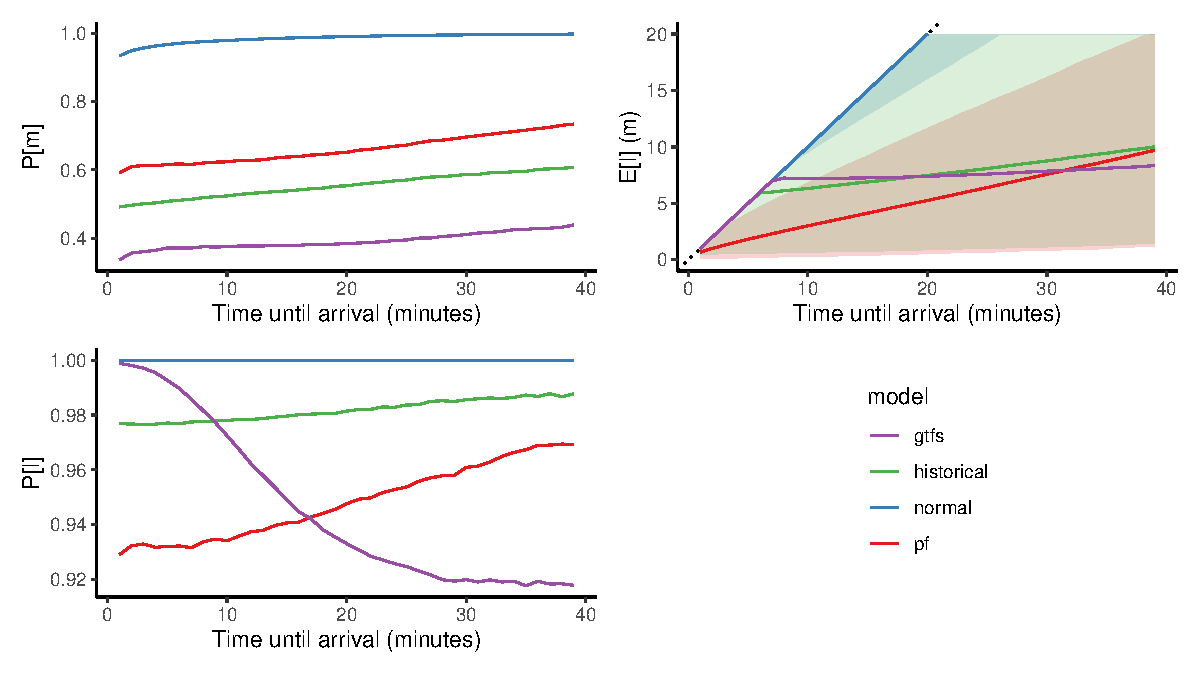
\includegraphics[width=\textwidth]{figure/model_results_pr_time-1} \caption[Summary values by time until arrival]{Summary values by time until arrival.}\label{fig:model_results_pr_time}
\end{figure}


\end{knitrout}


\subsubsection{Stop sequence}

Next, we computed the same values by stop sequence, as is shown in \cref{fig:model_results_pr_stop}. For most stops, the particle filter has a higher probability of the bus arriving after the point estimate ($\mathbb{P}_m$), though for early stops this is not the case. However, this is simply because the particle filter \emph{does not make a prediction} until the vehicle has been observed\footnote{Yet! Future work will work to use historical data in this situation}, whereas the \gls{gtfs} approach assumes the delay is zero until the vehicle is observed. This assumption can be reasonably accurate, particularly for the first few stops when there has not been enough time for the bus to get behind or ahead of schedule.

The trend for $\mathbb{P}_\ell$ is similar to what we saw with time until arrival. This time, however, the particle filter has much lower probabilities for the first few stops, again due to the reasons stated above. Even so, $\FM_4$ is consistently higher than $\FM_1$ until stop 40. The expected waiting time again shows better performance with the particle filter method until about stop 40, after which point the methods are more or less the same, given not many routes have over 40~stops. There is a trade-off here between waiting time and catch probability.


\begin{knitrout}\small
\definecolor{shadecolor}{rgb}{0.969, 0.969, 0.969}\color{fgcolor}\begin{figure}
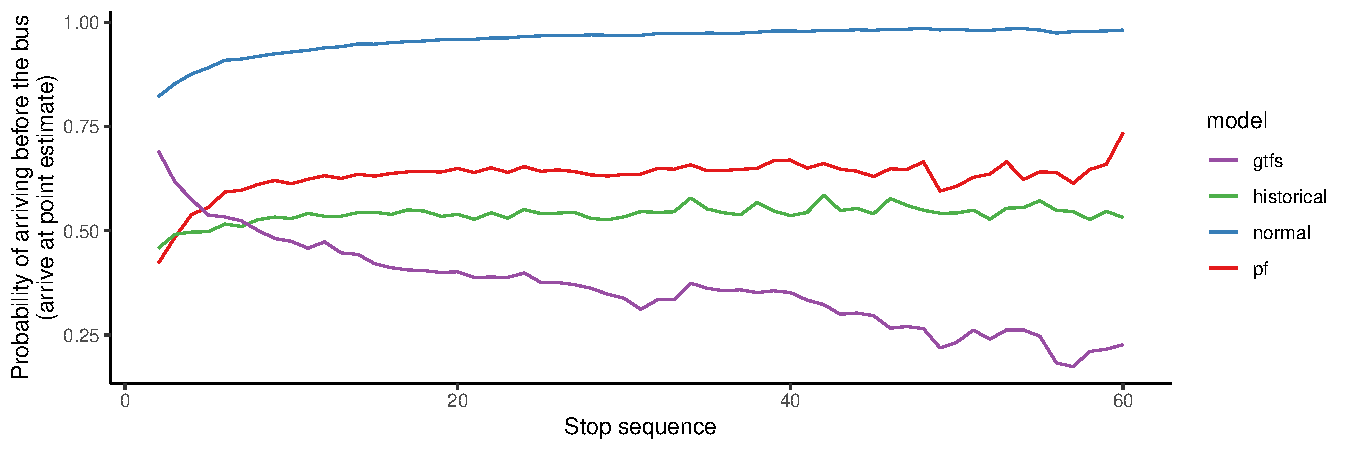
\includegraphics[width=\textwidth]{figure/model_results_pr_stop-1} \caption[Summary values by stop sequence]{Summary values by stop sequence.}\label{fig:model_results_pr_stop}
\end{figure}


\end{knitrout}


\subsubsection{Time of day}

Calculating the probabilities and expected waiting time in 15~minute intervals for each of the models is shown in \cref{fig:model_results_pr_timeofday}, in which the peak hour effects are visible, associated with an increased probability of arriving before the bus does in the particle filter method for both the median and lower bound. The schedule-delay method is negatively affected by peak hour in the lower bound estimate. The historical data estimate shows little effect due to peak hour but performs better in the day time (versus early morning and late evening).


For the expected waiting time, the particle filter is overall the lowest, even during peak where it shows a significant increase, seen in \cref{fig:model_results_pr_timeofday3}. The historical and schedule-delay methods both have similar expected waiting times of about 6--7 minutes.


\begin{knitrout}\small
\definecolor{shadecolor}{rgb}{0.969, 0.969, 0.969}\color{fgcolor}\begin{figure}
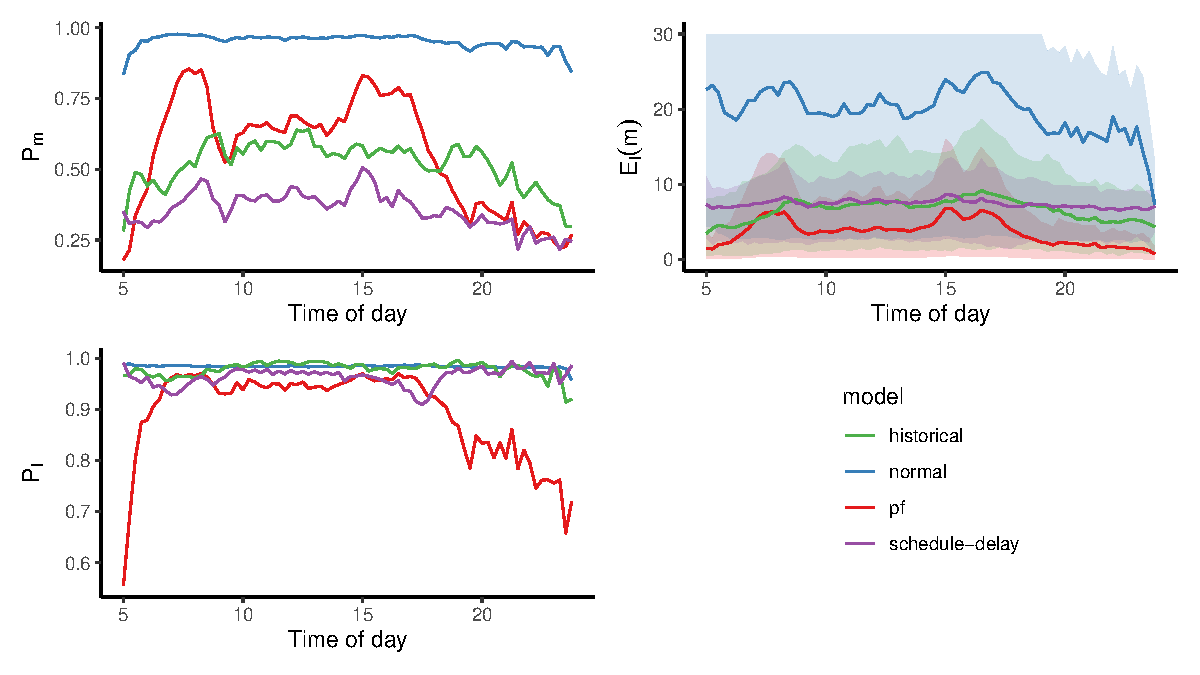
\includegraphics[width=\textwidth]{figure/model_results_pr_timeofday-1} \caption[Summary values by time of day]{Summary values by time of day.}\label{fig:model_results_pr_timeofday}
\end{figure}


\end{knitrout}



\subsection{Result summary}
\label{sec:prediction_model_comp_summary}

We have now seen that the particle filter suggests some improvement is possible over the schedule-delay method used by \AT. It tends to underestimate the arrival time, but even so, the expected waiting time is, in most situations, less than that of all of the other methods. Conversely, the normal approximation performed very poorly in this case, likely since summing uncertainties, and assuming independence, quickly results in an overestimation of uncertainty, and thus wide prediction intervals (not to mention high prediction error).

As for the other methods which do not use real-time network information, the historical data-based method performed as well as or better than the schedule-delay method, with a few situations where it did not perform so well. The average and variance of arrival delays were based on two weeks' worth of data, which is---at most---10 observations per trip. Processing more weeks of data could bring slight improvements, but without taking into account real-time data, it is unlikely to yield significant improvements. Post-processing is an intensive procedure, so future development could include real-time computation of the mean and variance of arrival time for each stop along each trip.

\section{Real-time performance}
\label{sec:prediction_performance}

The real-time performance of the our application has always been the main bottleneck, in that it needs to run in real-time and provide arrival time predictions as soon as possible after the data is received. During the simulation run to obtain the results from \cref{sec:prediction_model_comparison}, we also recorded the timings of individual parts of the program, of which overall averages are displayed in \cref{tab:prediction_timing}. In it, we have two timers: wall clock and CPU clock. Wall clock is the real-world time passed, while the CPU clock is the time spent on the processor.  We ran the simulation using four~cores, which affects the vehicle update (V) and \gls{eta} prediction (P) steps, as these are run in parallel. The other steps are not parallelised, so the wall and CPU timings are approximately similar, with the exception of the Load data (L) step, which involves calling the \gls{gtfs} \gls{api} and waiting for the data to download.


On average, the program takes less than five~seconds, which is well below our original target of 30~seconds. The most intensive component is updating of vehicle states, which involves updating 10,000 particles for each operating vehicle. This is followed by the \gls{eta} prediction step, which involves far fewer particles (we used 200 per trip), but each particle is required to estimate more per iteration [better wording]. However, the main advantage is that, in the vehicle update step, we perform a full weighted resample of the particles, which involves a full copy of all $\Np$ particles, plus sorting (if applicable). In the \gls{eta} step, we are able to use a single pointer to iterate over sampled particles, which completely avoids any copying.


\begin{knitrout}\small
\definecolor{shadecolor}{rgb}{0.969, 0.969, 0.969}\color{fgcolor}\begin{table}

\caption{\label{tab:prediction_timing}Time taken, in milliseconds, during various parts of the program, running on a single core.}
\centering
\fontsize{8}{10}\selectfont
\begin{tabular}[t]{lrlrl}
\toprule
 & Wall clock & (SE) & CPU time & (SE)\\
\midrule
(L) Load data & 29 & (0.21) & 17 & (0.19)\\
(U) Update vehicle information & 3.37 & (0.039) & 3.29 & (0.034)\\
(V) Vehicle state update & 3190 & (33) & 10300 & (97)\\
(N) Network state update & 0.458 & (0.012) & 1.35 & (0.026)\\
(P) Predict ETAs & 1310 & (27) & 3170 & (37)\\
\addlinespace
(W) Write ETAs to protobuf feed & 162 & (0.57) & 189 & (0.53)\\
\midrule
(T) Total iteration time & 4690 & (51) & 13700 & (130)\\
\bottomrule
\end{tabular}
\end{table}


\end{knitrout}


However, there is a high level of variability in the number of buses operating at any given time (figure X), so in \cref{fig:prediction_timing_time} we have displayed the timings for each individual iteration over the course of the day. We again see the peak hour effect, where there are upwards of 1000~vehicles operating. This pushes the total iteration time to a between 10 and 15~seconds, which is still well within our target of 30~seconds. We could slightly increase the number of particles, although it is worth remembering that the \emph{resampling} step of the particle filter has a computational complexity of $\mathcal{O}(N\log N)$, so for example we cannot double the number of particles and expect to remain under the 30~second target.
\textcolor{red}{Note to self: re-run simulations overnight, when you're not also using the CPU cores for other tasks, which should remove the oddity between about 9am and 2pm.}


\begin{knitrout}\small
\definecolor{shadecolor}{rgb}{0.969, 0.969, 0.969}\color{fgcolor}\begin{figure}

{\centering 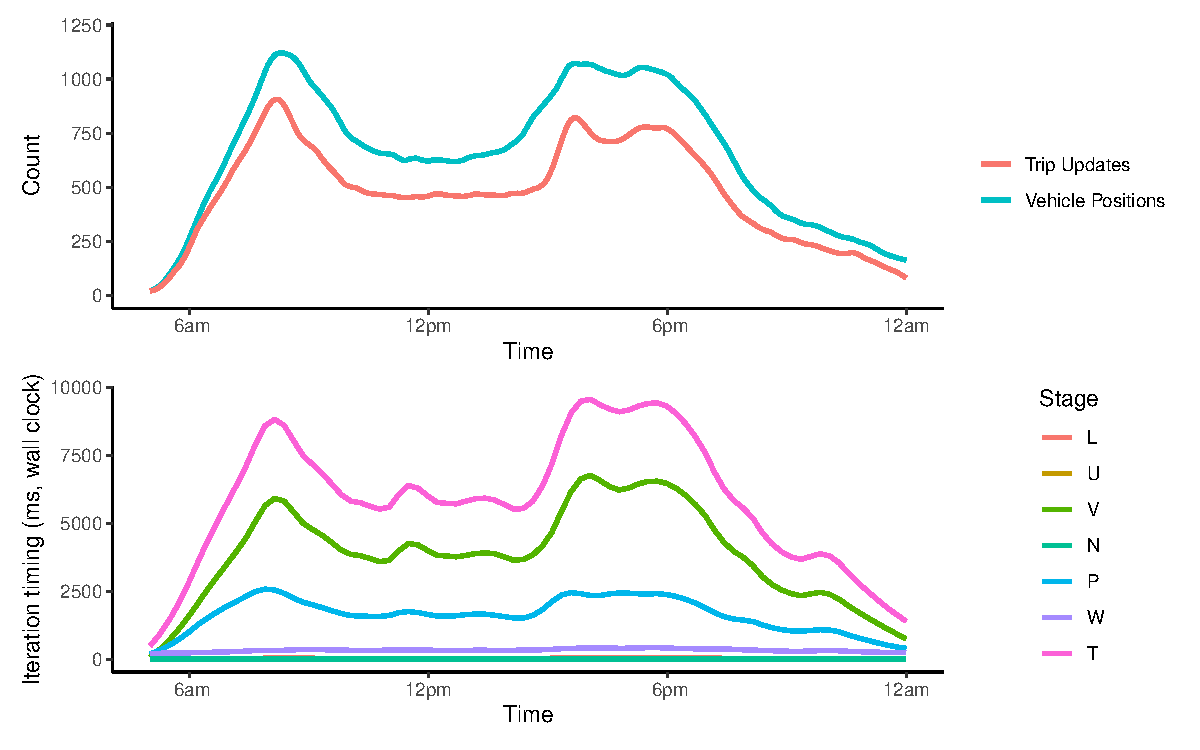
\includegraphics[width=\textwidth]{figure/prediction_timing_time-1} 

}

\caption[Number of vehicles and trip updates at different times ofthe day, along with the timing results over time for various stages of the program]{Number of vehicles and trip updates at different times ofthe day, along with the timing results over time for various stages of the program: (L) Load data, (O) Update vehicles information, (V) Vehicle state update, (N) Network state update, (P) Predict ETAs, (W) Write ETAs to protobuf feed, (T) Total iteration time.}\label{fig:prediction_timing_time}
\end{figure}


\end{knitrout}

